%\begin{mydef}
%	Deux droites sont \kw{sécantes} si elles n'ont qu'un seul point commun : leur \kw{point d'intersection}.
%\end{mydef}
%
%
%\begin{myex}
%	\begin{multicols}{2}
%		Les droites $(d)$ et $(d')$ sont sécantes en $O$ qui est leur point d'intersection.
%		
%		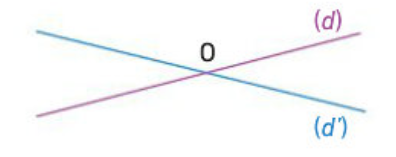
\includegraphics[scale=0.5]{img/sec}
%	\end{multicols}
%	
%\end{myex}
%
%\begin{mydef}
%	Deux droites sont \kw{perpendiculaires} si elles se coupent en formant \kw{quatre angles droits}. Si deux droites $(d_1)$ et $(d_2)$ sont deux droites perpendiculaires, on note $(d_1) \perp (d_2)$.
%\end{mydef}
%
%\begin{myex}
%	\begin{multicols}{2}
%		Les droites $(d)$ et $(d')$ sont perpendiculaires en $H$. $H$ est le pied de la perpendiculaire à $(d')$.
%		
%		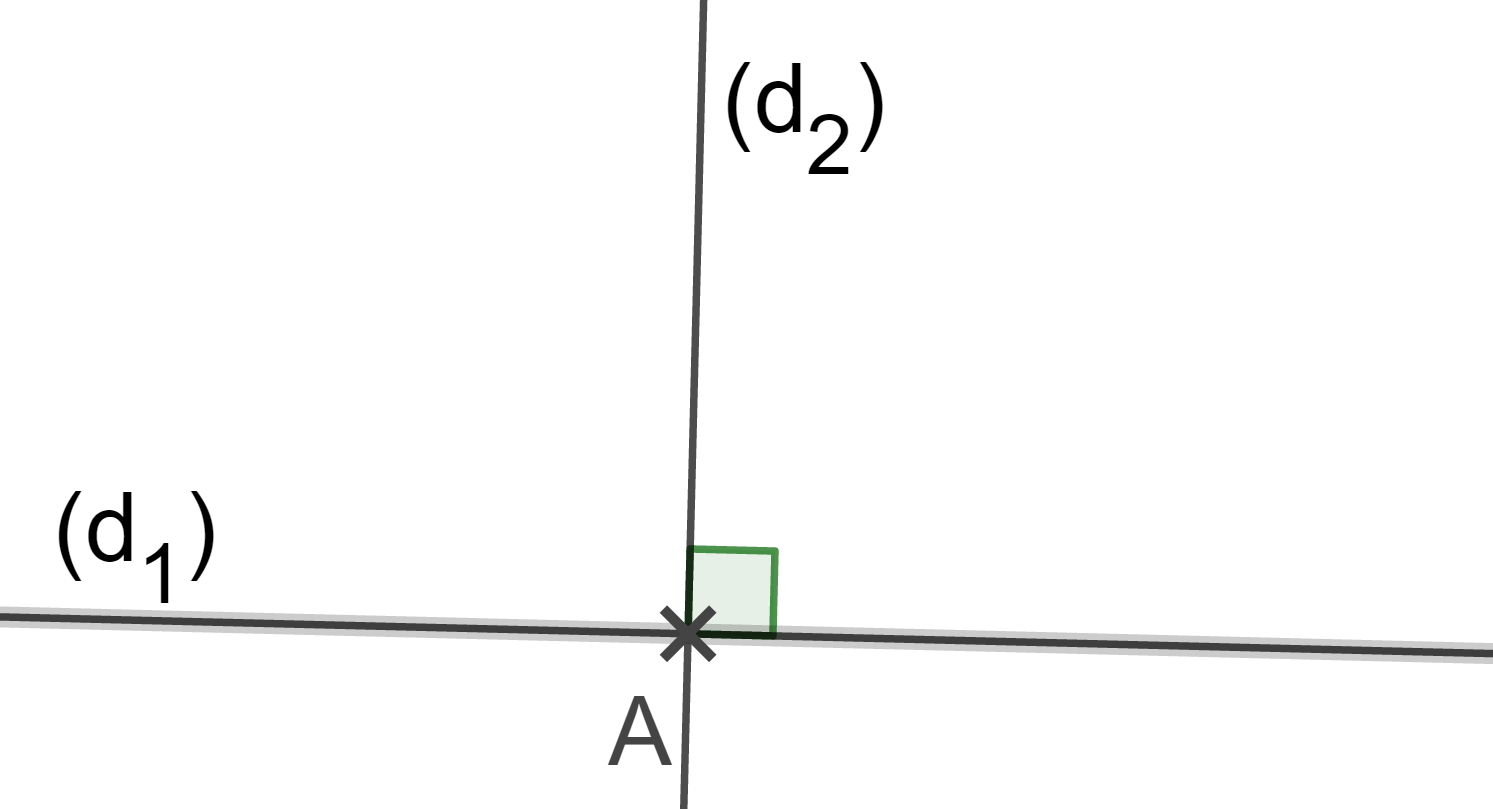
\includegraphics[scale=0.6]{img/perp}
%	\end{multicols}
%	
%\end{myex}
%
%\begin{mydef}
%	Deux droites qui ne sont pas sécantes sont \kw{parallèles}. Si deux droites $(d_3)$ et $(d_4)$ sont parallèles, on note $(d_1) // (d_2)$.
%\end{mydef}
%
%\begin{myex}
%	\begin{multicols}{2}
%		Les droites $(d)$ et $(d')$ sont parallèles. Même en les prolongeant à l'infini elles ne se rencontreront jamais.
%		
%		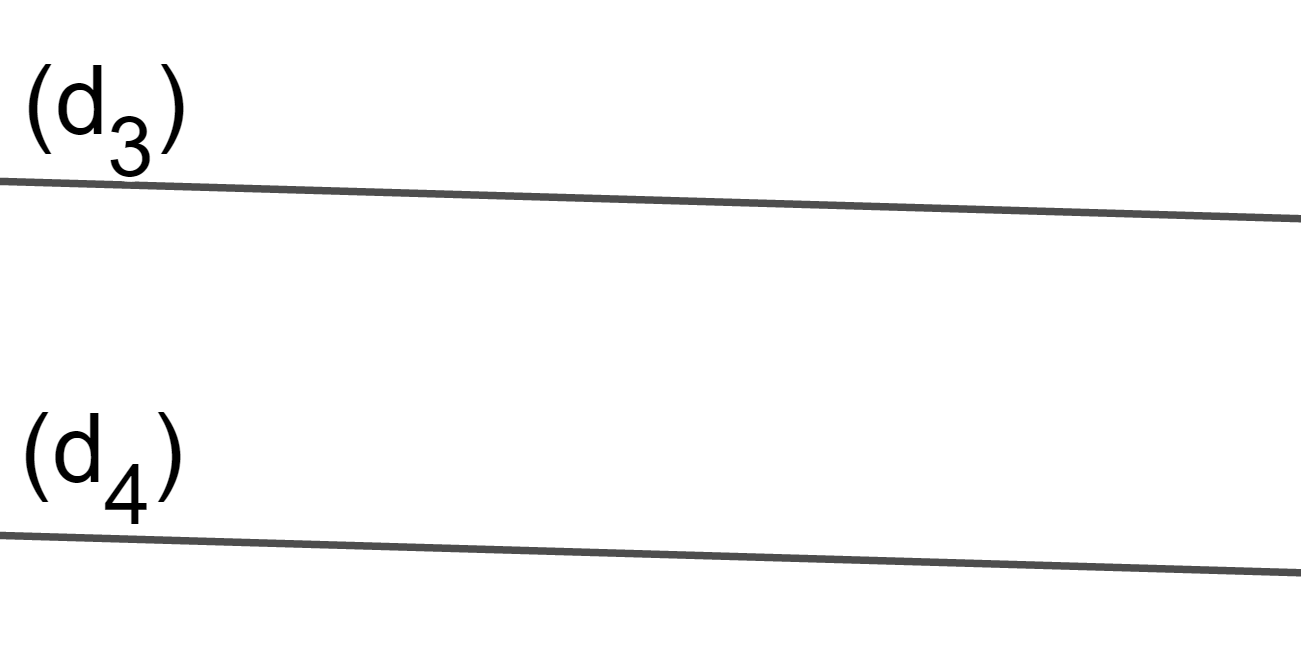
\includegraphics[scale=0.6]{img/para1}
%	\end{multicols}
%	
%\end{myex}
%
%\begin{myprop}
%	\kw{Si} deux droites sont perpendiculaires à une même troisième droite, \kw{alors} ces deux droites sont parallèles.
%\end{myprop}
%
%
%\begin{myex}
%	\begin{multicols}{2}
%		\kw{On sait que} $(d_1)$ et $(d_2)$ sont toutes deux perpendiculaires à $(D)$.\\
%		\kw{Donc} $(d_1)$ et $(d_2)$ sont parallèles.
%		
%		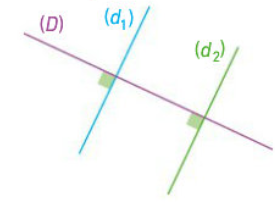
\includegraphics[scale=0.6]{img/para2}
%	\end{multicols}
%	
%\end{myex}



\begin{myprop}
	\kw{Si} deux droites sont parallèles, \kw{alors} toute perpendiculaire à l’une est perpendiculaire à l’autre
\end{myprop}


\begin{myex}
	\begin{multicols}{2}
		\kw{On sait que} $(d_1)$ // $(d_2)$ et $(d_1) \perp (D)$\\
		\kw{Donc} $(d_2) \perp (D)$.
		
		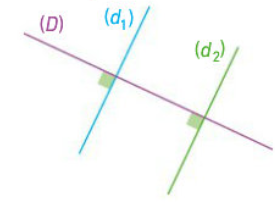
\includegraphics[scale=0.6]{img/para2}
	\end{multicols}
	
\end{myex}

\begin{myprop}
	\kw{Si} deux droites sont parallèles à une même troisième, \kw{alors} ces deux droites sont parallèles entre elles.
\end{myprop}

\begin{myex}
	\begin{multicols}{2}
		\kw{On sait que} $(d_1)$ // $(d)$ et $(d_2) // (d)$\\
		\kw{Donc} $(d_1) \perp (d_2)$.
		
		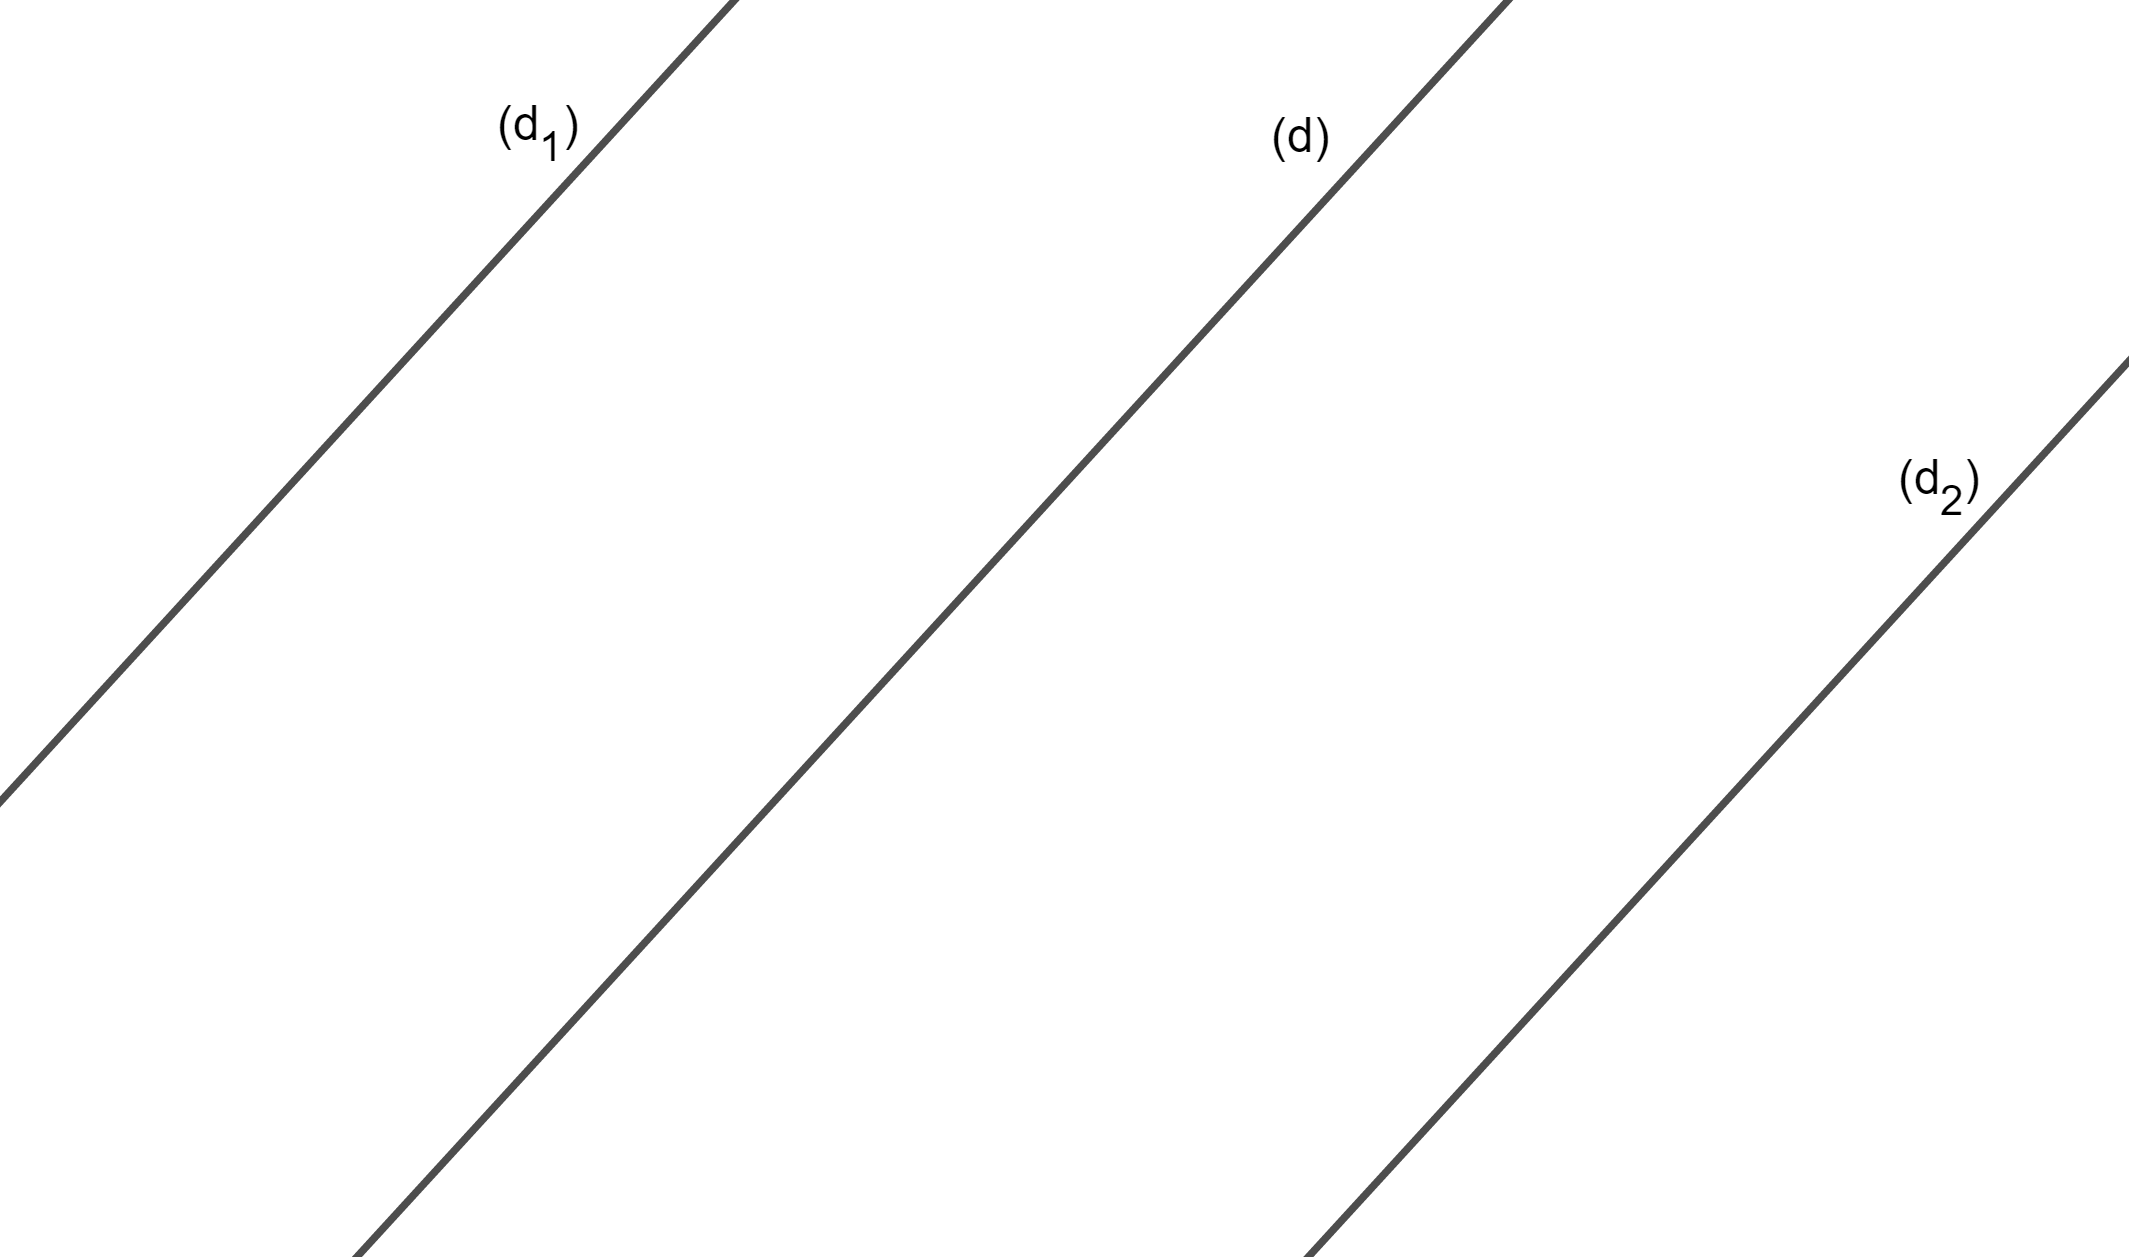
\includegraphics[scale=0.1]{img/para3}
	\end{multicols}
	
\end{myex}
